\epi{I have this phobia about having my body penetrated surgically. You
know what I mean?}{\textit{eXistenZ}\\\textsc{TED PIKUL}}
\noindent{}
\gomarginpar{The following text is from \cite{go_interfaces}. Written by Ian 
Lance Taylor --- one of the authors of Go.}
In Go, the word \first{\emph{interface}}{interface} is overloaded to mean several different
things. Every type has an interface, which is the \emph{set of methods
defined} for \index{interface!set of methods}
that type. This bit of code defines a struct type \type{S} with one field, and
defines two methods for \type{S}.
\begin{lstlisting}[caption=Defining a struct and methods on it,label=src:interface object]
type S struct { i int }
func (p *S) Get() int { return p.i }
func (p *S) Put(v int) { p.i = v }
\end{lstlisting}
You can also define an \first{interface type}{interface!type}, which is simply a set of methods.
This defines an interface \type{I} with two methods:
\begin{lstlisting}
type I interface {
  Get() int
  Put(int)
}
\end{lstlisting}

\noindent\type{S} is a valid \emph{implementation} for interface \type{I}, because it defines the two 
methods which \type{I} requires. Note that this is true even though there is 
no explicit declaration that \type{S} implements \type{I}. 

A Go program can use 
this fact via yet another meaning of interface, which is an
\first{interface value}{interface!value}:

\begin{lstlisting}
func f(p I) {  |\longremark{Declare a function that takes an interface type %
as the argument;}|
    fmt.Println(p.Get()) |\longremark{As \var{p} implements interface \type{I} %
it \emph{must} have the \func{Get()} method;}|
    p.Put(1) |\longremark{Same holds for the \func{Put()} method.}|
}
\end{lstlisting}
\showremarks
Here the variable \var{p} holds a value of interface type. Because
\type{S} implements \type{I}, we can call \func{f} passing in a pointer to a 
value of type \type{S}:
\begin{lstlisting}
var s S; f(&s)
\end{lstlisting}

The reason we need to take the address of \type{s}, rather than a value of type
\type{S}, is because we defined the methods on \type{s} to operate on
pointers, see the code above in listing \ref{src:interface object}.
This is not a requirement --- we could have defined the methods to take
values --- but then the \func{Put} method would not work as expected.

The fact that you do not need to declare whether or not a type implements an
interface means that Go implements a form of 
\first{duck typing}{duck typing}\cite{duck_typing}. 
This is not
pure duck typing, because when possible the Go compiler will statically
check whether the type implements the interface. However, Go does have a
purely dynamic aspect, in that you can convert from one interface type
to another. In the general case, that conversion is checked at runtime.
If the conversion is invalid --- if the type of the value stored in the
existing interface value does not satisfy the interface to which it is
being converted --- the program will fail with a runtime error.

Interfaces in Go are similar to ideas in several other programming languages:
pure abstract virtual base classes in C++, typeclasses in Haskell or duck typing
in Python. However there is no other language which combines
interface values, static type checking, dynamic runtime conversion, and no
requirement for explicitly declaring that a type satisfies an interface. The
result in Go is powerful, flexible, efficient, and easy to write.

\subsection{Which is what?}
Lets define another type that also implements the interface \type{I}:
\begin{lstlisting}
type R struct { i int }
func (p *R) Get() int { return p.i }
func (p *R) Put(v int) { p.i = v }
\end{lstlisting}
The function \func{f} can now accept variables of type \type{R} and \type{S}.
Suppose you need to know the actual type in the function \func{f}. In Go you can 
figure that out by using a \first{type switch}{type switch}.

\begin{lstlisting}
func f(p I) {
    switch t := p.(type) { |\longremark{The type switch. Use \key{(type)} in a \key{switch} %
statement. We store the type in the variable \var{t};}|
        case *S: |\longremark{The actual type of \var{p} is a pointer to \type{S};}|
        case *R: |\longremark{The actual type of \var{p} is a pointer to \type{R};}|
        case S:  |\longremark{The actual type of \var{p} is a \type{S};}|
        case R:  |\longremark{The actual type of \var{p} is a \type{R};}|
        default: |\longremark{It's another type that implements \type{I}.}|
    }
}
\end{lstlisting}
\showremarks
Using \key{(type)} outside a \key{switch} is illegal. A type switch isn't the only way
to discover the type at \emph{run-time}. 
You can also use a "comma, ok" form to see if an interface type implements
a specific interface:

\begin{lstlisting}
if t, ok := any.(I); ok { 
   // any implements the interface I
   // t is the type it has
} 
\end{lstlisting}
When you are sure a variable implements an interface you can use:
\begin{lstlisting}
t := any.(I)
\end{lstlisting}

\subsection{Empty interface}
Since every type satisfies the empty interface:
\type{interface\{\}}. We can create a generic function which 
has an empty interface as its argument:
\begin{lstlisting}[caption=A function with an empty interface argument,label=src:interface empty]
func g(any interface{}) int { 
    return any.(I).Get() 
}
\end{lstlisting}
The \lstinline{return any.(I).Get()} is the tricky bit in this function.
The value \var{any} has type \type{interface\{\}}, meaning no guarantee
of any methods at all: it could contain any type. The \lstinline{.(I)}
is a \first{type assertion}{type assertion} which converts \var{any} to an interface of
type \type{I}. If we have that type we can invoke the \func{Get()}
function.
So if we create a new variable of the type \type{*S}, we can just
call \func{g()}, because \type{*S} also implements the empty interface.
\begin{lstlisting}
s = new(S)
fmt.Println(g(s));
\end{lstlisting}
The call to \func{g} will work fine and will print 0. If we however
invoke \func{g()} with a value that does not implement \type{I} we have
a problem:
\begin{lstlisting}[caption=Failing to implement an interface,label=src:interface fail]
i := 5		|\coderemark{Make i a "lousy" \texttt{int}}|
fmt.Println(g(i))
\end{lstlisting}
This compiles, but when we run this we get slammed with:

\noindent\error{panic: interface conversion: int is not main.I: missing
method Get}

\noindent{}Which is completely true, the built-in type \type{int} does not
have a \func{Get()} method.

\section{Methods}
Methods are functions that have an receiver (see chapter
\ref{chap:functions}).
You can define methods on any type (except on non-local types, this includes
built-in types: the type \type{int} can not have methods).
You can however make a new integer type with its own methods. For example:
\begin{lstlisting}
type Foo int

func (self Foo) Emit() {
  fmt.Printf("%v", self)
}

type Emitter interface {
  Emit()
}
\end{lstlisting}
Doing this on non-local (types defined in other packages) types yields:
% Empty line here is critical, otherwise no new paragraph is created

\begin{minipage}{.5\textwidth}
\begin{lstlisting}[linewidth=.7\textwidth,caption=Failure extending built-in types]
func (i int) Emit() {
  fmt.Printf("%d", i)
}
\end{lstlisting}
\noindent\error{cannot define new methods\\ on non-local type int}
\end{minipage}
\begin{minipage}{.5\textwidth}
\begin{lstlisting}[caption=Failure extending non-local types]
func (a *net.AddrError) Emit() {
  fmt.Printf("%v", a)
}
\end{lstlisting}
\noindent\error{cannot define new methods\\ on non-local type net.AddrError}
\end{minipage}

\paragraph{}  %% needed otherwise the minipage flows over

\subsection{Methods on interface types}
An interfaces defines a set of methods. A method contains the actual code.
In other words, an interface is the definition and the methods are the implementation.
So a receiver can not be a defined for interface
types, doing so results in a \error{invalid receiver type ...} compiler
error. The authoritative word from the language spec \cite{go_spec}:
\begin{quote}
The receiver type must be of the form \type{T} or \type{*T} where
\type{T} is a type name. \type{T} is called the receiver base type or just base 
type. The base type must
not be a pointer or interface type and must be declared in the same
package as the method.
\end{quote}

\begin{lbar}[Pointers to interfaces]
Creating a pointer to an interface value is a useless action in Go.
It is in fact illegal to
create a pointer to an interface value. The release notes for the release \gorelease{2010-10-13}
that
made them illegal leave no room for doubt:
\begin{quote}
The language change is that uses of pointers to interface values no longer 
automatically dereference the pointer.  A pointer to an interface value is more 
often a beginner's bug than correct code.
\end{quote}
From the \cite{go_faq}. If not for this restriction, this code:
\begin{lstlisting}
var buf bytes.Buffer
io.Copy(buf, os.Stdin)
\end{lstlisting}
Would copy standard input into a copy of \var{buf}, not into \var{buf} itself. 
This is almost never the desired behavior.
\end{lbar}

\section{Interface names}
By convention, one-method interfaces are named by the method name plus
the \emph{-er} suffix: Read\emph{er}, Writ\emph{er}, Formatt\emph{er} etc.

There are a number of such names and it's productive to honor them and
the function names they capture. \func{Read}, \func{Write},
\func{Close}, \func{Flush}, \func{String} and
so on have canonical signatures and meanings. To avoid confusion, don't
give your method one of those names unless it has the same signature and
meaning. Conversely, if your type implements a method with the same
meaning as a method on a well-known type, give it the same name and
signature; call your string-converter method \func{String} not
\func{ToString}.
\gomarginpar{Text copied from \cite{effective_go}.}

\section{A sorting example}
\label{sec:a sorting example}
Recall the Bubblesort exercise (Q\ref{ex:bubble}), where we sorted an
array of integers:
\begin{lstlisting}
func bubblesort(n []int) {
    for i := 0; i < len(n)-1; i++ {
	for j := i + 1; j < len(n); j++ {
	    if n[j] < n[i] {
		    n[i], n[j] = n[j], n[i]
	    }
	}
    }
}
\end{lstlisting}
A version that sorts strings is identical except for the signature of
the function:
\begin{lstlisting}
func bubblesortString(n []string) { /* ... */ }
\end{lstlisting}
Using this approach would lead to two functions, one for each type. By using
interfaces we can make this more \index{generic} generic.
Lets create a new function that will sort both strings and
integers, something along the lines of this non-working example:
\begin{lstlisting}
func sort(i []interface{}) { |\longremark{Our function will receive a slice of %
empty interfaces;}|
    switch i.(type) {        |\longremark{Using a type switch we find out what the %
actual type is of the input;}|
	case string:         |\longremark{And then sort accordingly;}|
	    // ...
	case int:
	    // ...
    }
    return /* ... */ |\longremark{Return the sorted slice.}|
}
\end{lstlisting}
\showremarks
But when we call this function with \lstinline|sort([]int{1, 4, 5})|, it
fails with:\\
\noindent\error{cannot use i (type []int) as type []interface { } in function argument}

This is because Go can not easily convert to a \emph{slice} of interfaces.
Just converting to an interface is easy, but to a slice is much more costly.
To keep a 
\gomarginpar{The full mailing list discussion on this subject
can be found at \cite{go_nuts_interfaces}.}
long story short: Go does not (implicitly) convert slices for you.

So what is the Go way of creating such a "generic" function? 
Instead of doing the type inference our selves with a type switch, we let
Go do it implicitly:
The following steps are required:
\begin{enumerate}
\item Define an interface type (called \type{Sorter} here) with a number of 
methods needed for sorting.
We will at least need a function to get the length of the slice,
a function to compare two values and a swap function;
\begin{lstlisting}
type Sorter interface {
    Len() int           |\coderemark{\texttt{len()} as a method}|
    Less(i, j int) bool |\coderemark{\texttt{p[j] $<$ p[i]} as a method}|
    Swap(i, j int)      |\coderemark{\texttt{p[i], p[j] = p[j], p[i]} as a method}|
}
\end{lstlisting}
\item Define new types for the slices we want to sort. Note that we
declare slice types;
\begin{lstlisting}
type Xi []int
type Xs []string
\end{lstlisting}
\item Implementation of the methods of the \type{Sorter} interface.
For integers:
\begin{lstlisting}
func (p Xi) Len() int               { return len(p) }
func (p Xi) Less(i int, j int) bool { return p[j] < p[i] }
func (p Xi) Swap(i int, j int)      { p[i], p[j] = p[j], p[i] }
\end{lstlisting}
And for strings:
\begin{lstlisting}
func (p Xs) Len() int               { return len(p) }
func (p Xs) Less(i int, j int) bool { return p[j] < p[i] }
func (p Xs) Swap(i int, j int)      { p[i], p[j] = p[j], p[i] }
\end{lstlisting}
\item Write a \emph{generic} Sort function that works on the \type{Sorter} interface.
\begin{lstlisting}
func Sort(x Sorter) { |\longremark{\var{x} is now of the \texttt{Sorter} type;}|
    for i := 0; i < x.Len() - 1; i++ { |\longremark{Using the defined functions, we implement Bubblesort.}|
	for j := i + 1; j < x.Len(); j++ {
	    if x.Less(i, j) {
		x.Swap(i, j)
	    }
	}
    }
}
\end{lstlisting}
\showremarks
\end{enumerate}
We can now use you generic \func{Sort} function as follows:
\begin{lstlisting}
ints := Xi{44, 67, 3, 17, 89, 10, 73, 9, 14, 8}
strings := Xs{"nut", "ape", "elephant", "zoo", "go"}

Sort(ints)
fmt.Printf("%v\n", ints)
Sort(strings)
fmt.Printf("%v\n", strings)
\end{lstlisting}

\subsection{Listing interfaces in interfaces}
Take a look at the following example of an interface defintion, this one is 
from the package \package{container/heap}:
\begin{lstlisting}
type Interface interface {
    sort.Interface
    Push(x interface{})
    Pop() interface{}
}
\end{lstlisting}
Here another interface is listed inside the definition of \type{heap.Interface}, this
may look odd, but is perfectly valid, remember that on the surface an interface is nothing
more than a listing of methods. \type{sort.Interface} is also such a listing, so it is
perfectly legal to include it in the interface.

\subsection{Introspection and reflection}
\label{sec:introspection and reflection}
In the following example we want to look at the "tag" (here named
"namestr") defined in the
type definition of \type{Person}. To do this we need the
\package{reflect}\index{package!reflect} package (there is no other way in Go). Keep in mind
that looking at a tag means going back the \emph{type} definition. So
we use the \package{reflect} package to figure out the type of the variable
and \emph{then} access the tag.

\begin{lstlisting}[caption=Introspection using reflection,label=src:introspection]
|\begin{tikzpicture}[overlay]
\draw [->,thick] (2.8,-6.00) node [left] %
{\longremark{We are dealing with a \type{PtrValue} and according %
to the documentation\footnote{\texttt{godoc reflect}}:%
\begin{quote} %
\texttt{\func{func} (v *PtrValue) Elem() Value}\\%
Elem returns the value that v points to. %
If v is a nil pointer, Elem returns a nil Value. %
\end{quote} %
we can use \func{Elem()} to get the type the pointer points to. %
In this case \type{*reflect.StructValue};}} %
to (2.8,-5.20);
%
\draw [->,thick] (3.8,-6.00) node [left] %
{\longremark{\func{Type()} returns \type{reflect.Type};}} %
to (3.8,-5.20);
\draw [->,thick] (5.4,-6.00) node [left] %
{\longremark{%
Again according to the documentation, we have:\\%
\begin{quote} %
\ldots which returns an object with interface %
type \type{Type}.  That contains a pointer to a struct of type %
\type{*StructType}, %
\type{*IntType}, etc. representing the details of the underlying type. %
A type switch or type assertion can reveal which. %
\end{quote} %
So we can access your specific type as a member of this struct. Which %
we do with \type{(*reflect.StructType)};}} %
to (5.4,-5.20);
%
\draw [->,thick] (6.8,-6.00) node [left] %
{\longremark{%
A \type{StructType} has a number of methods, one of which is %
\func{Field($n$)} which returns the $n^{th}$ field of a structure. %
The type of this return is a \type{StructField}; %
}} %
to (6.8,-5.20);
%
\draw [->,thick] (8.4,-6.00) node [left] %
{\longremark{We finally have the type we are after. Now we can use the %
methods defined for \type{*StructType}, like \func{Field(n)}, which %
returns the n$^{th}$ field of our struct as a \type{StructField};}} %
to (8.4,-5.20);
%
\draw [->,thick] (9.4,-6.00) node [left] %
{\longremark{The struct \type{StructField} has a \var{Tag} member which %
returns the tag-name as a string. So on the $0^{th}$ field we can %
unleash \func{.Tag} to access this name: \texttt{Field(0).Tag}. This %
\emph{finally} gives us \texttt{namestr}.}}%
to (9.4,-5.20);
\end{tikzpicture}|
type Person {
    name string "namestr"
    age  int
}

p1 := new(Person)   |\coderemark{\func{new} returns a pointer to Person}|
ShowTag(p1)	    |\coderemark{\func{ShowTag()} is now called with this pointer}|

func ShowTag(i interface{}) {
    switch t := reflect.NewValue(i).(type) { |\coderemark{Type assertion}|
    case *reflect.PtrValue:		     |\coderemark{\var{p1} is a pointer}|
	tag := t.Elem().Type().(||*reflect.StructType).Field(0).Tag
||
\end{lstlisting}

\showremarks

%% look at layout
To make the difference between types and values more clear,
that a look at the following code:
\begin{lstlisting}[caption=Reflection and the type and value]
func show(i interface{}) {
    switch t := i.(type) {
      case *Person:
        t := reflect.TypeOf(i)  |\coderemark{Go for type meta data}|
        v := reflect.ValueOf(i) |\coderemark{Go for the actual values}|
	tag := t.Elem().Field(0).Tag |\longremark{Here we want to get to the "tag". %
So we need \func{Elem()} to redirect the pointer, access the first field and get the tag. %
Note we operate on \var{t} a \type{reflect.Type};}|
	name := v.Elem().Field(0).String() |\longremark{Now we want to get access to the %
\emph{value} of one of the members and we %
employ\newline\lstinline{Elem()} on \var{v} to do the redirection. %
Now we have arrived at the structure. Then we go the the first field %
\lstinline{Field(0)} and invoke the \lstinline{String()} method on %
it. %
\begin{figure}[H] %
\hskip3\baselineskip\parbox{0.7\textwidth}{\caption[Peeling away the layers using reflection]{Peeling away the %
layers using reflection. %
Going from a \type{*Person} via \mbox{\func{Elem()}} using the %
methods described in \prog{godoc reflect} to get the %
actual \type{string} contained within.}} %
\label{fig:reflection} %
\begin{center} %
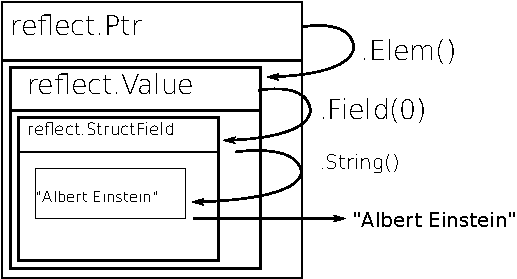
\includegraphics[scale=0.75]{fig/reflection.pdf} %
\end{center}\end{figure} %
}|
    }
}
\end{lstlisting}
\showremarks

Setting a value works similarly as getting a value, but only works on
\emph{exported} members. Again some code:

\begin{minipage}{.5\textwidth}
\begin{lstlisting}[caption=Reflect with private member]
type Person struct {
 name string "namestr" |\coderemark{name}|
 age  int
}

func Set(i interface{}) {
 switch i.(type) {
 case *Person:
  r := reflect.ValueOf(i)
  r.Elem(0).Field(0).SetString("Albert Einstein")
  }
}
\end{lstlisting}
\end{minipage}
\hspace{2em}
\begin{minipage}{.5\textwidth}
\begin{lstlisting}[caption=Reflect with public member]
type Person struct {
 Name string "namestr" |\coderemark{\emph{N}ame}|
 age  int
}

func Set(i interface{}) {
 switch i.(type) {
 case *Person:
  r := reflect.ValueOf(i)
  r.Elem().Field(0).SetString("Albert Einstein")
  }
}
\end{lstlisting}
\end{minipage}
The code on the left compiles and runs, but when you run it, you are greeted with a
stack trace and a \emph{runtime} error:

\noindent\error{panic: reflect.Value.SetString using value obtained using unexported field}

\noindent{}The code on the right works OK and sets the member \var{Name}
to "Albert Einstein". Of course this only works when you call \func{Set()}
with a pointer argument.

\section{Exercises}
\begin{Exercise}[title={接口和编译},difficulty=1]
\Question
在第 \pageref{src:interface fail} 页的代码 \ref{src:interface fail} 
编译正常——就像文中开始描述的那样。但是当运行的时候,会得到运行时错误,
因此有些东西\emph{有}错误。为什么代码编译没有问题呢?
\end{Exercise}

\begin{Answer}
\Question
代码能够编译是因为整数类型实现了空接口,这是在编译时检查的。

修复这个正确的途径是测试这个空接口可以被转换,如果可以,调用对应的方法。
\ref{src:interface empty} 列出的 Go 代码中定义了函数 \func{g}——这里重复一下:
\begin{lstlisting}
func g(any interface{}) int { return any.(I).Get() }
\end{lstlisting}

\noindent{}应当修改为:
\begin{lstlisting}
func g(any interface{}) int {
    if v, ok := any.(I); ok {	// 检查是否可以转换
	return v.Get()		// 如果可以,调用 Get()
    }
    return -1			// 随便返回个什么
}
\end{lstlisting}
如果现在调用 \func{g()},就不会有运行时错误了。在 Go 中这种用法被称作``comma ok''。
\end{Answer}


\begin{Exercise}[title={Pointers and reflection},difficulty=5]
\label{ex:pointers and reflection}
\Question
One of the last paragraphs in section "\titleref{subsec:introspection and reflection}" 
on page \pageref{subsec:introspection and reflection}, has
the following words:
\begin{quote}
The code on the right works OK and sets the member \var{Name}
to "Albert Einstein". Of course this only works when you call \func{Set()}
with a pointer argument.
\end{quote}
Why is this the case?
\end{Exercise}

\begin{Answer}
\Question
When called with a non-pointer argument the variable is a copy (call-by-value). So you
are doing the reflection voodoo on a copy. And thus you are \emph{not}
changing the original value, but only this copy.
\end{Answer}


\begin{Exercise}[title={接口和最大最小},difficulty=1]
\Question
构造一个通用的最大最小,使得可以同时工作于整数和字符串,就像第 \titleref{sec:a sorting example} 节中那样。
\end{Exercise}

\begin{Answer}
\Question
\end{Answer}


\cleardoublepage
\section{Answers}
\shipoutAnswer
